% !TEX TS-program = xelatex
% !TEX encoding = UTF-8 Unicode

% 雖然這裡把浮水印跟DOI在LaTeX內直接加入的功能保留(預設為關閉),
% 但強烈建議大家還是使用Acobat或Foxit PDF Reader手動嫁入,
% 避免格式跑掉,然後被圖書館找碴。

\documentclass[
  degree        = master,               % degree = master | doctor
  language      = chinese,              % language = chinese | english
  watermark     = false,                % watermark = true | false
  doi           = false,                % doi = true | false
  AutoFakeSlant = 0.25,
  AutoFakeBold  = 2
]{ntuthesis}

% !TeX root = ./main.tex

% --------------------------------------------------
% 資訊設定(Information Configs)
% --------------------------------------------------

\ntusetup{
  university*   = {National Taiwan University},
  university    = {國立臺灣大學},
  college       = {社會科學院},
  college*      = {College of Social Sciences},
  institute     = {政治學系},
  institute*    = {Department of Poliotical Science},
  title         = {無詠唱魔法理論基礎},
  title*        = {Theoretical Foundations of Non-chanted Magic},
  author        = {魯迪烏斯·格雷拉特},
  author*       = {Rudeus Greyrat},
  ID            = {R09322008},
  advisor       = {洛琪希·米格路迪亞·格雷拉特},
  advisor*      = {Roxy Migurdia Greyrat},
  date          = {2023-08-01},         % 若註解掉,則預設為當天
  oral-date     = {2023-08-01},         % 若註解掉,則預設為當天
  DOI           = {10.5566/NTU2018XXXXX},
  keywords      = {LaTeX, 中文, 論文, 模板},
  keywords*     = {LaTeX, CJK, Thesis, Template},
}

% --------------------------------------------------
% 加載套件(Include Packages)
% --------------------------------------------------

\usepackage[style = apa, 
            backend = biber, 
            natbib]{biblatex}           % 參考文獻      
\usepackage{paralist}                   % 列表環境
\usepackage{lipsum}                     % 英文亂字
\usepackage{zhlipsum}                   % 中文亂字
\usepackage{url}
\usepackage{adjustbox}                  % 圖表縮放
\usepackage{threeparttable}             % 複雜圖表環境
\usepackage{rotating}                   % 表格水平轉置
\usepackage{tablefootnote}              % 表格內註解
\usepackage{xcolor}                     % 顏色RGB
\usepackage{tikz}                       % LaTeX畫圖
\usepackage{makecell}
\usepackage{enumitem}

% \usepackage[capposition = top]{floatrow}

% --------------------------------------------------
% 套件設定(Packages Settings)
% --------------------------------------------------

\addbibresource{back/references.bib}         % 參考文獻資源庫
\usetikzlibrary{shapes, arrows, positioning} % LaTeX畫圖資源庫

% 自訂數學符號
\DeclareMathOperator*{\argmin}{arg\,min}

% 自調表格種類
\newcolumntype{L}[1]{>{\raggedright\let\newline\\\arraybackslash\hspace{0pt}}m{#1}}
\newcolumntype{C}[1]{>{\centering\let\newline\\\arraybackslash\hspace{0pt}}m{#1}}
\newcolumntype{R}[1]{>{\raggedleft\let\newline\\\arraybackslash\hspace{0pt}}m{#1}}


\begin{document}

% 封面與口試審定
% Cover and Verification Letter
\frontmatter
\makecover                                     % 論文封面(Cover)
\makeverification{./front/verification.pdf}    % 口試委員審定書(Verification Letter)

% 致謝與論文摘要
% Acknowledgement and Abstract
% !TeX root = ../main.tex

\begin{acknowledgement}

我已經能夠走向外界。她成功達成沒有任何人能辦到的事情。這是生前,父母跟兄弟們都沒能辦到的事情。洛琪希卻幫我辦到了。不是靠不負責任的空口白話,而是扛起責任帶給我勇氣。她並非刻意這麼做。我很清楚。她是為了自己。這點我也知道。不過,我還是該尊敬她。要尊敬那位嬌小的少女。我在內心發誓,目送洛琪希的背影遠去直到完全消失。手裡只剩下她送我的魔杖跟項鏈。還有許許多多的知識。--- \textit{\Kai 《無職轉生》,第一卷}

\end{acknowledgement}           % 致謝(Acknowledgement)
% !TeX root = ../main.tex

\begin{abstract}

中文摘要中文摘要中文摘要中文摘要中文摘要中文摘要中文摘要中文摘要中文摘要中文摘要中文摘要中文摘要中文摘要中文摘要中文摘要中文摘要中文摘要中文摘要中文摘要中文摘要中文摘要中文摘要中文摘要中文摘要中文摘要中文摘要中文摘要中文摘要中文摘要中文摘要中文摘要中文摘要中文摘要中文摘要中文摘要中文摘要中文摘要中文摘要中文摘要中文摘要中文摘要中文摘要中文摘要中文摘要中文摘要中文摘要中文摘要中文摘要中文摘要中文摘要中文摘要中文摘要中文摘要中文摘要中文摘要中文摘要中文摘要中文摘要中文摘要中文摘要中文摘要中文摘要中文摘要中文摘要中文摘要中文摘要中文摘要中文摘要中文摘要中文摘要中文摘要中文摘要中文摘要中文摘要中文摘要中文摘要中文摘要中文摘要中文摘要

\end{abstract}

\begin{abstract*}

\lipsum[1]

\end{abstract*}                  % 摘要(Abstract)

% 生成目錄與符號列表
% Contents of Tables and Denotation
\maketableofcontents                    % 目錄(Table of Contents)
\makelistoffigures                      % 圖目錄(List of Figures)
\makelistoftables                       % 表目錄(List of Tables)

% 論文內容
% Contents of Thesis
\mainmatter
% !TeX root = ../main.tex

\chapter{緒論}

\section{文件說明}

這個模板根據\href{https://github.com/Hsins}{Hsins}大的\href{https://github.com/Hsins/NTU-Thesis-LaTeX-Template}{NTU-Thesis-LaTeX-Template}所修改而來,並供臺大政治系研究生利用\href{https://www.latex-project.org}{\LaTeX}撰寫論文。這個版本的模板大致上仍為持Hsins大所設計架構,並只有在以下幾處進行格式上的調整來更符合政治系的論文格式。你可以在我的\href{https://github.com/withworksc/NTUPS_Thesis_Template}{Github專案}中下載原始碼\footnote{\texttt{href}字的顏色預設仍為黑色,如果有需要可以到cls裡面加回來。}。
% !TeX root = ../main.tex

\chapter{文獻回顧}

\section{英文引用測試}

\lipsum[2]\citep{hetherington_2001_partisan,layman_geoffrey_2002_conflict,layman_et_al_2006_polar,zaller_1992_mass,iyengar_et_al_2012_affective,iyengar_et_al_2019_affective}.

\section{中文引用測試}

以下為中文引用\citep{sheng_2010_longtitude,chen_et_al_2009_cross,hawang_2004_legi,sheng_2003_compare,juang_et_al_2017_curroption,}。
% !TeX root = ../main.tex

\chapter{研究設計與方法}

\section{模型設定}

M-Estimation的目標試如等式\eqref{eq:m_esti}所示:
\begin{equation}
\label{eq:m_esti}
\hat{\theta} = \argmin_{\theta \in \Theta} \sum_{i = 1}^n \nabla_{\theta} q (w_i, \theta) \triangleq \argmin_{\theta \in \Theta} \sum_{i = 1}^n s_i(\theta)
\end{equation}


% !TeX root = ../main.tex

\chapter{實證結果}

\section{插入圖表}


% Table created by stargazer v.5.2.2 by Marek Hlavac, Harvard University. E-mail: hlavac at fas.harvard.edu
% Date and time: Wed, May 12, 2021 - 23:43:54
\begin{table}[!htbp] \centering 
  \caption{迴歸報表範例} 
  \label{tb:regTable} 
\begin{tabular}{@{\extracolsep{5pt}}lcccc} 
\\[-1.8ex]\hline 
\hline \\[-1.8ex] 
 & \multicolumn{4}{c}{\textit{Dependent variable:}} \\ 
\cline{2-5} 
\\[-1.8ex] & \multicolumn{4}{c}{logRent} \\ 
 & POLS & RE & FE & FD \\ 
\\[-1.8ex] & (1) & (2) & (3) & (4)\\ 
\hline \\[-1.8ex] 
 y90 & 0.262$^{***}$ & 0.323$^{***}$ & 0.386$^{***}$ &  \\ 
  & (0.035) & (0.029) & (0.037) &  \\ 
  & & & & \\ 
 logPop & 0.041$^{*}$ & 0.056$^{*}$ & 0.072 & 0.072 \\ 
  & (0.023) & (0.029) & (0.088) & (0.088) \\ 
  & & & & \\ 
 logAvgInc & 0.571$^{***}$ & 0.447$^{***}$ & 0.310$^{***}$ & 0.310$^{***}$ \\ 
  & (0.053) & (0.052) & (0.066) & (0.066) \\ 
  & & & & \\ 
 pctstu & 0.005$^{***}$ & 0.005$^{***}$ & 0.011$^{***}$ & 0.011$^{***}$ \\ 
  & (0.001) & (0.001) & (0.004) & (0.004) \\ 
  & & & & \\ 
 Constant & $-$0.569 & 0.445 &  & 0.386$^{***}$ \\ 
  & (0.535) & (0.566) &  & (0.037) \\ 
  & & & & \\ 
\hline \\[-1.8ex] 
Observations & 128 & 128 & 128 & 64 \\ 
Adjusted R$^{2}$ & 0.857 & 0.949 & 0.950 & 0.288 \\ 
\hline 
\hline \\[-1.8ex] 
\textit{Note:}  & \multicolumn{4}{r}{$^{*}$p$<$0.1; $^{**}$p$<$0.05; $^{***}$p$<$0.01} \\ 
\end{tabular} 
\end{table} 


\begin{figure}[!htbp]
\centering
\caption{全台家戶薪資分布,按村里}
\label{fig:income}
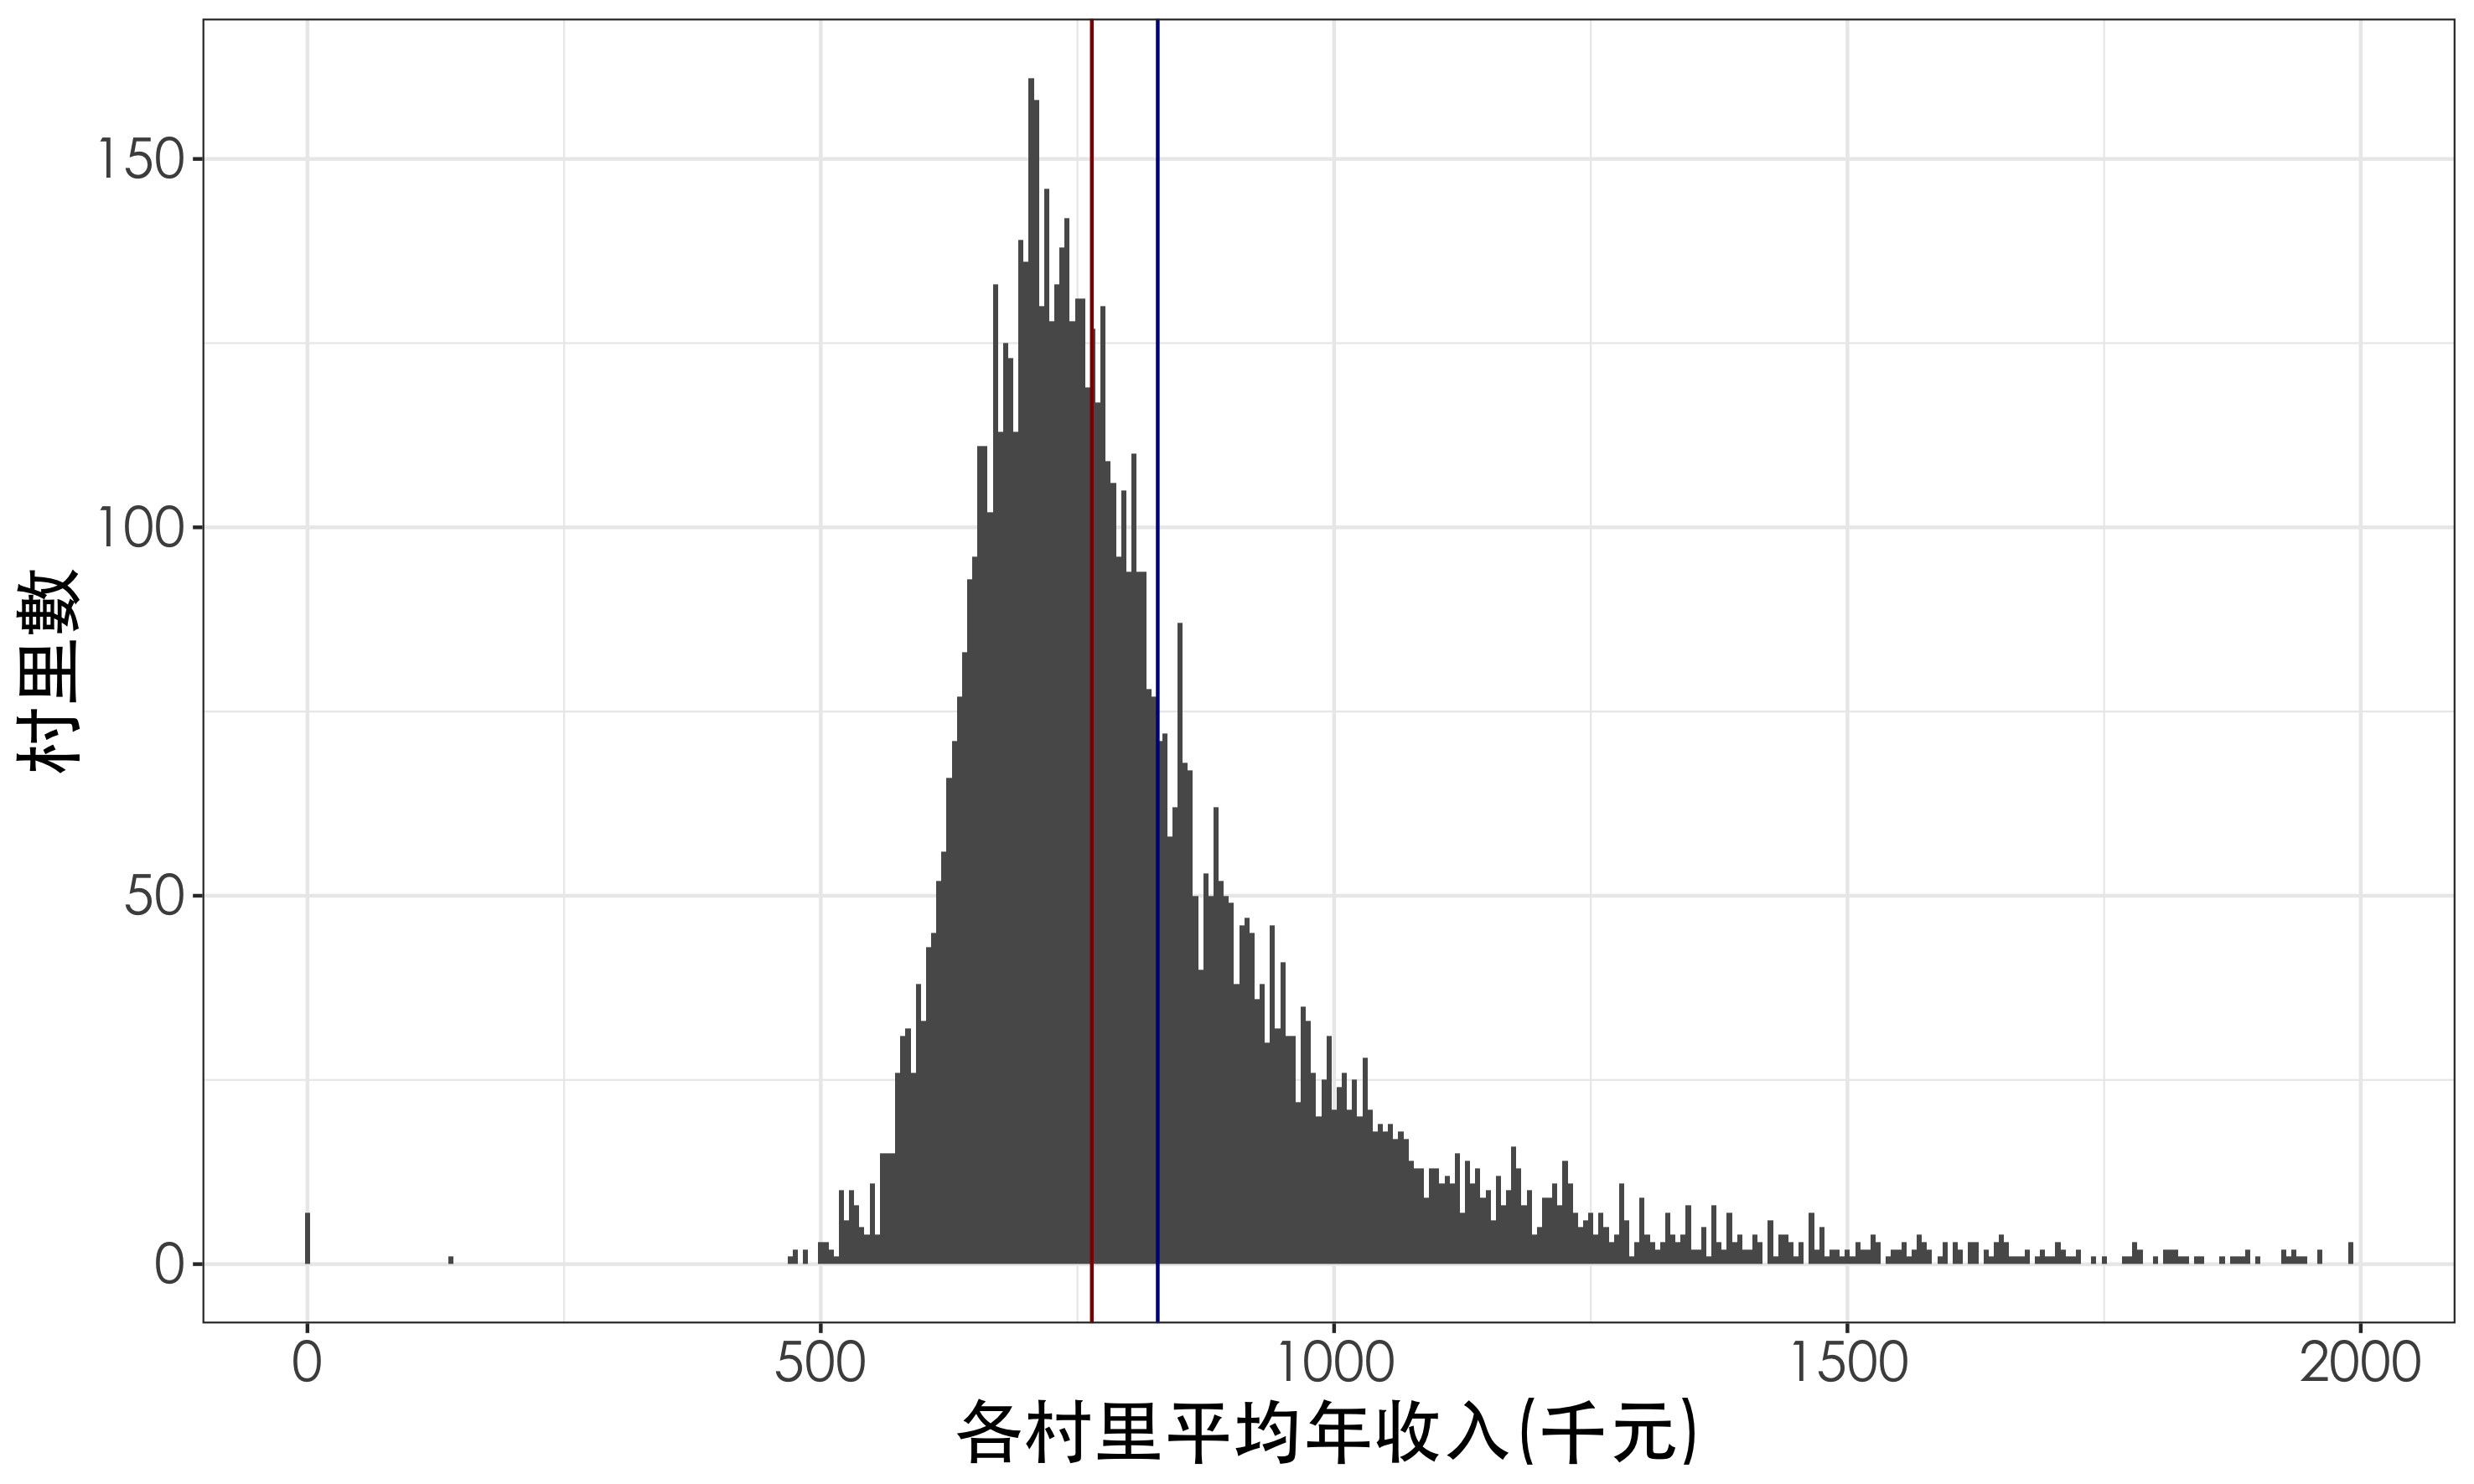
\includegraphics[width = \textwidth]{contents/figures/township_income.png}
\end{figure}



% 參考文獻
% References
\refmatter
% \printbibliography                   % <- 你可以直接把中英的參考文獻混再一起

\printbibheading                       % <- 或者分中文與英文兩部分,但記得在reference.bib中要加入keyword
\section*{一、英文部分}
\printbibliography[keyword = {english}, heading = none]
\section*{二、中文部分}
\printbibliography[keyword = {chinese}, heading = none]

% 附錄
% Appendices
% !TeX root = ../main.tex

\appendix{A}{這是附錄}
\section{附錄段落1}
\section{附錄段落2}

% \input{back/appendix02}               % <- 我先把原有的附錄先註解到了,你如果需要可以再重新加回

\end{document}
